% Document Class is specified here. We're using the Homework Template
\documentclass[12pt, a4paper]{article}

\usepackage{graphicx}
\usepackage{float}
\usepackage{geometry}
\usepackage{verbatim}
\usepackage{listings}

\lstset{
  basicstyle=\itshape,
  xleftmargin=3em,
  literate={->}{$\rightarrow$}{2}
           {ε}{$\epsilon$}{1}
}

\geometry{a4paper, margin=1in}

\title{Week 5 CS-312 Homework}
\author{
	Cory Ness
	\and
	Jack Engledow
	\and
	James Sgrazzutti
}

\begin{document}

\maketitle

\section{Problem 6.6}
\subsection{Question}
Give CFG's for the following languages with alphabet $\{a,b\}$:
\subsubsection{All strings of the form $a^{m}b^{n}$ with $m \leq n \leq 2m$.}
\begin{lstlisting}
S -> ε | aSB 
B -> b | bb
\end{lstlisting}
\subsubsection{All strings such that the middle symbol is $a$.}
\begin{lstlisting}
S -> aSa | aSb | bSb | bSa | a
\end{lstlisting}

\section{Problem 6.10}
\subsection{Question}
Consider the following CFG with start variable $S$:
\begin{lstlisting}
S -> BB
B -> SS | c
\end{lstlisting}
\subsubsection{What is the shortest string in the language of the grammar?}
\begin{center}
$cc$
\end{center}
\subsubsection{Draw the derivation tree for the string from (2.1.1).}
\begin{center}
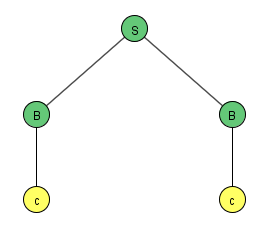
\includegraphics[scale=1]{6.10.b}
\end{center}
\subsubsection{Is this grammar ambiguous? Explain.}
Yes, because in the case of $ccccc$ (5 $c$'s), the derivation can be achieved either by splitting the first $B$ or the second $B$ into $SS$.
\subsubsection{Describe in English the language generated by the grammar.}
Any string with 2mod3 number of $c$'s.
\subsubsection{Does this CFG generate a regular language? Explain.}
Yes, because the equivalent regular expression is $cc(ccc)^{*}$

\section{Problem 6.11}
\subsection{Question}
Describe in English the language generated by the following grammar:
\begin{lstlisting}
S -> 0S1 | 1S0 | ε | SS
\end{lstlisting}
Sketch a proof that your answer is correct.
\subsection{Answer}
This language is any string with an equal number of $0$'s and $1$'s.\newline
\newline
We can prove this by looking at every string's first and last symbol, solving it, removing it, and moving on to the inward set of symbols in the string.\newline
For a string $0w1$ or $1w0$, the string can be broken into $w$ using the rule $S \to 0S1$ or $S \to 1S0$. For a string $0w0$ or $1w1$, there must also be a $1s1$ or $0s0$ that is inside the $w$. This can be rewritten as $0u1j1u0$, which can be broken up into $0u1$, $j$, and $1u0$ by $S \to SS$. These individual parts are part of the grammar, and so any string with an equal number of $0$'s and $1$'s is accepted.

\section{Problem 7.6}
\subsection{Question}
Explain how, given a PDA for $L_{1}$ and a PDA for $L_{2}$, you can produce a PDA for hte concatenation $L_{1}L_{2}$.
\subsection{Answer}
Create a Grammar for both $L_{1}$ and $L_{2}$, called $G_{1}$ and $G_{2}$. Concatenate the grammars, so that $G \to G_{1}G_{2}$. Convert $G$ back into a PDA.

\section{Problem 7.9}
\subsection{Question}
Construct a PDA for the language of binary strings with an unequal number of $0$'s and $1$'s.
\subsection{Answer}
\begin{center}
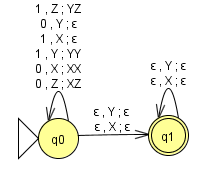
\includegraphics[scale=1]{7.9}
\end{center}

\section{Problem 7.13}
\subsection{Question}
Consider the language of strings where (at least) the first half is all the same symbol. To be specific, consider the set of all string $a^{n}x$ where $|x| \leq n$ and $x \in \{a,b\}^{*}$. Give both a grammar and a PDA for this language.
\subsection{Answer}
\begin{lstlisting}
S -> aST | ε
T -> a | b | ε
\end{lstlisting}
\begin{center}
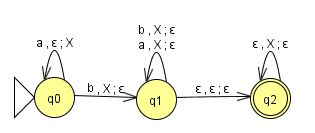
\includegraphics[scale=1]{7.13}
\end{center}


\end{document}